\chapter{SYSTEM ANALYSIS}

\section{Introduction}
System analysis is the process of studying a procedure or business to identify its goals and purposes and create systems and procedures that will achieve them in an efficient way. In this phase, we dive deep into "what" the system must do to solve the civic reporting crisis.

\section{Module Description}
The "CivicGuard" application is architected into several functional modules, each handling a distinct part of the application logic:
\begin{itemize}
    \item \textbf{User Authentication \& Profile Management:} This module manages the core security layer using Laravel's robust authentication scaffolding. It supports secure registration, password hashing (Bcrypt), and session management. Role-based access control (RBAC) ensures that citizens are restricted to reporting functions while officers can access departmental tasks.
    \item \textbf{Report Lifecycle Module:} The engine that manages the ingestion and state of damage reports. It handles multi-part form validation, asynchronous photo uploads, and status transitions. Each report is treated as a state machine, moving from "Pending" to "Assigned" and finally "Repaired" upon verification.
    \item \textbf{Intelligent Routing Engine:} A backend logic layer that automatically parses report categories (e.g., "Pothole" $\rightarrow$ "Roads Dept") to find the correct municipal body. This decoupling ensures that routing rules can be updated dynamically without modifying the frontend submission logic.
    \item \textbf{Personalized Dashboards:} Highly dynamic views built with Blade that provide "Glance-at-a-glance" status updates. Citizens view their submission history and resolution rates, while officers receive a prioritized queue of unresolved tasks within their ward.
    \item \textbf{Real-Time Notification Engine:} Leveraging Laravel's event system, this module triggers alerts (Email/Dashboard) when a report changes status. This ensures that the reporting citizen is notified the moment an officer starts an inspection or completes a repair.
\end{itemize}

\section{Project Development Timeline}
The project was executed over a span of 12 weeks, following an Agile approach. The table below outlines the timeline for various development sprints and milestones.

\begin{table}[H]
\centering
\renewcommand{\arraystretch}{1.3}
\begin{tabular}{|c|p{4cm}|p{9cm}|}
\hline
\textbf{Week} & \textbf{Sprint Name} & \textbf{Core Accomplishments} \\ \hline
1-2 & Inception & Initial research, feasibility study, and environment setup. \\ \hline
3-4 & Alpha Sprint & Core authentication and user profile logic development. \\ \hline
5-7 & Beta Sprint & Implementation of reporting lifecycle and department routing. \\ \hline
8-9 & Gamma Sprint & Frontend refinement, dashboard orchestration, and analytics. \\ \hline
10-11 & QA Sprint & Detailed unit, integration, and system testing. \\ \hline
12 & Delivery & Final documentation, report generation, and deployment. \\ \hline
\end{tabular}
\caption{CivicGuard Project Development Timeline}
\label{tab:timeline}
\end{table}

\section{Business Rules \& Logic}
The system is governed by a strict set of business rules to ensure accountability:
\begin{itemize}
    \item \textbf{Visibility Rule:} Data visibility is strictly partitioned by role. Officers see only their department's data to prevent information overload and ensure focus.
    \item \textbf{Verification Rule:} A report CANNOT be closed (marked as Repaired) without the upload of a "Resolution Photo." This prevents false claims of completion.
    \item \textbf{Audit Rule:} Every status change is logged with a timestamp and the ID of the officer who performed it, creating a full audit trail.
\end{itemize}

\section{Feasibility Study}
A prerequisite to development, the feasibility study evaluates the project's viability:

\subsection{Technical Feasibility}
The system is highly feasible as it uses the PHP 8.2+ and Laravel 11.x stack, which are industry standards for robust web applications. The hardware required to host the system is modest (4GB RAM, 10GB storage), making it compatible with existing municipal servers or low-cost cloud providers. Furthermore, the use of open-source tools ensures that there are no recurring licensing fees for the core software stack.

\subsection{Economic Feasibility}
From an economic standpoint, CivicGuard is a high-return investment. By digitizing the reporting process, it eliminates the need for manual record-keeping and reduces the administrative hours spent on routing complaints. More importantly, early identification of infrastructure damage (e.g., fixing a small leak before it bursts) results in significant cost savings for the municipality by preventing major asset failures.

\subsection{Social \& Operational Feasibility}
Socially, the platform empowers citizens by giving them a transparent voice in urban maintenance, fostering a "Digital Democracy" environment. Operationally, the system integrates seamlessly into existing workflows; officers receive tasks directly on their dashboards, removing the need for physical memos or phone calls to initiate repairs.

\begin{table}[H]
\centering
\renewcommand{\arraystretch}{1.5}
\begin{tabular}{|p{4cm}|p{3cm}|p{7cm}|}
\hline
\textbf{Feasibility Category} & \textbf{Status} & \textbf{Key Justification} \\ \hline
\textbf{Technical} & High & Uses standardized PHP/Laravel stack; low hardware overhead. \\ \hline
\textbf{Economic} & Positive & Long-term savings through automated routing and proactive maintenance. \\ \hline
\textbf{Social} & High & Encourages citizen participation and builds trust through transparency. \\ \hline
\textbf{Operational} & Excellent & Seamlessly digitizes existing manual workflows with RBAC security. \\ \hline
\end{tabular}
\caption{Comprehensive Feasibility Analysis Summary}
\label{tab:feasibility_summary}
\end{table}

\section{System Requirements}
To ensure optimal performance and stability, the CivicGuard system requires the following hardware and software configurations for both development and production environments.

\subsection{Hardware Requirements}
The following hardware specifications are recommended to handle the concurrent reporting traffic and image processing tasks effectively.
\begin{table}[H]
\centering
\renewcommand{\arraystretch}{1.5}
\begin{tabular}{|p{4cm}|p{10cm}|}
\hline
\textbf{Component} & \textbf{Minimum Specification} \\ \hline
\textbf{Processor (CPU)} & Modern multi-core processor (Intel Core i3/AMD Ryzen 3 or higher) for rendering complex DOM elements and executing background jobs smoothly. \\ \hline
\textbf{Memory (RAM)} & 4 GB (8 GB recommended for heavy WebSocket usage and parsing large images locally). \\ \hline
\textbf{Storage} & Minimum 10 GB of free space for database storage, caching, and hosting uploaded user evidence photos. \\ \hline
\textbf{Display} & A screen resolution of 1366x768 or higher is recommended for the responsive dashboard layout. \\ \hline
\textbf{Network} & A stable internet connection is required for real-time status updates and notification broadcasting. \\ \hline
\end{tabular}
\caption{System Hardware Requirements}
\label{tab:hw_req}
\end{table}

\subsection{Software Requirements}
The software stack is built on modern open-source technologies to ensure high compatibility and long-term support.
\begin{table}[H]
\centering
\renewcommand{\arraystretch}{1.5}
\begin{tabular}{|p{4cm}|p{10cm}|}
\hline
\textbf{Software} & \textbf{Specification / Version} \\ \hline
\textbf{Operating System} & Windows 10/11, macOS, or Linux (Ubuntu/Debian recommended for server). \\ \hline
\textbf{Web Server} & Apache 2.4 or Nginx 1.20+ \\ \hline
\textbf{Language} & PHP 8.2 or higher (required for Laravel 11 features). \\ \hline
\textbf{Database} & PostgreSQL 14.0 \\ \hline
\textbf{Package Manager} & Composer 2.x and NPM (Node.js 18+) \\ \hline
\textbf{Web Browser} & Modern browsers (Chrome, Firefox, Safari, Edge) with JavaScript enabled. \\ \hline
\end{tabular}
\caption{System Software Stack Requirements}
\label{tab:sw_req}
\end{table}

\section{Requirement Analysis}

\subsection{Functional Requirements}
\begin{table}[H]
\centering
\renewcommand{\arraystretch}{1.3}
\begin{tabular}{|c|p{4cm}|p{8cm}|}
\hline
\textbf{Req ID} & \textbf{Feature} & \textbf{Description} \\ \hline
FR01 & User Registration & Allow residents to create accounts with email and contact details. \\ \hline
FR02 & Incident Reporting & Enable photo upload, category selection, and location tagging. \\ \hline
FR03 & Auto-Assignment & Map reports to the correct department based on category logic. \\ \hline
FR04 & Status Tracking & Real-time dashboard updates for Citizens and Officers. \\ \hline
FR05 & Admin Control & Tools for user management and system-wide announcements. \\ \hline
\end{tabular}
\caption{Functional Requirements Specification}
\label{tab:func_req}
\end{table}

\subsection{Non-Functional Requirements}
To ensure that the system is not only functional but also reliable and user-friendly, the following non-functional requirements have been established:
\begin{itemize}
    \item \textbf{Usability:} The interface must be intuitive, allowing a first-time user to submit a report in under 2 minutes.
    \item \textbf{Performance:} Page load times for the dashboard should not exceed 2 seconds under normal network conditions.
    \item \textbf{Security:} All passwords must be hashed using Bcrypt, and sessions must expire after 30 minutes of inactivity.
    \item \textbf{Scalability:} The system architecture must support up to 50 concurrent image uploads without significant degradation in service.
\end{itemize}

\section{Actors and Roles}
The CivicGuard system involves three primary groups of stakeholders, each with specific permissions and responsibilities:
\begin{itemize}
    \item \textbf{Citizen:} The primary user who identifies and reports public asset damage. They can register, log in, submit reports with photos, and track the status of their grievances.
    \item \textbf{Departmental Officer:} Authorized personnel from municipal departments (e.g., Electricity, Roads). They receive routed reports, perform inspections, update repair statuses, and upload resolution proof.
    \item \textbf{Administrator:} The system overseer who manages user roles, moderates public content, and analyzes high-level reporting trends for municipal planning.
\end{itemize}

\section{Use Case Model}
The Use Case model defines the functional requirements of the CivicGuard system from the perspective of its users. It illustrates the various ways in which actors interact with the system to achieve their specific goals.

\begin{figure}[H]
    \centering
    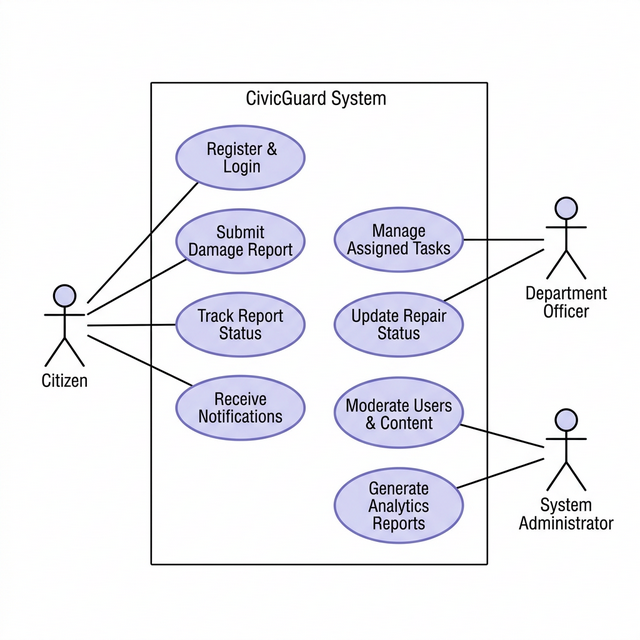
\includegraphics[width=0.85\textwidth]{images/use_case_diagram.png}
    \caption{UML Use Case Diagram - System Functionality Overview}
    \label{fig:use_case}
\end{figure}

The diagram above provides a high-level view of the system's core capabilities. Citizens primarily focus on the reporting lifecycle, while departmental officers and administrators manage the backend processing and system governance. This visual mapping ensures that every functional requirement is directly linked to an authorized user role.

\subsection{Use Case Descriptions}
The following table provides a detailed breakdown of the primary use cases identified in the diagram, specifying the prerequisites and expected outcomes for each interaction.

\begin{longtable}{|p{1.5cm}|p{2.5cm}|p{2cm}|p{3.5cm}|p{2.5cm}|p{2.5cm}|}
\hline
\textbf{UC ID} & \textbf{Use Case} & \textbf{Primary Actor} & \textbf{Description} & \textbf{Pre-condition} & \textbf{Post-condition} \\ \hline
\endfirsthead
\hline
\textbf{UC ID} & \textbf{Use Case} & \textbf{Primary Actor} & \textbf{Description} & \textbf{Pre-condition} & \textbf{Post-condition} \\ \hline
\endhead
\hline
\endfoot
\hline
\endlastfoot
UC01 & Register & Citizen & Allows new users to create a system identity. & User has a valid email address. & Account is created and stored in DB. \\ \hline
UC02 & Login & All & Authenticates users based on credentials. & User is already registered. & Session is established with role. \\ \hline
UC03 & Submit Report & Citizen & Ingestion of damage report with photos. & User is logged in as Citizen. & Report is saved with 'Pending' status. \\ \hline
UC04 & View Dashboard & All & Provides role-specific data overview. & User is authenticated. & Personalized cards/tables rendered. \\ \hline
UC05 & Assign Department & System & Auto-routes report to correct body. & Report is submitted successfully. & Report linked to dept officer. \\ \hline
UC06 & Update Status & Officer & Changes report state (e.g. to In-Progress). & Report is assigned to the officer. & Status updated; log entry created. \\ \hline
UC07 & Upload Proof & Officer & Submits resolution photo for verification. & Repair is physically complete. & Resolution photo stored & linked. \\ \hline
UC08 & Moderation & Admin & Managing users and system-wide settings. & User has Admin privileges. & Audit trail logged; changes live. \\ \hline
\caption{Detailed Use Case Descriptions}
\label{tab:uc_descriptions}
\end{longtable}
